\chapter{Mapping over Quartic and Sextic twisted KSS Curves}
\label{ch:ijnc2017}
\section{Introduction}
\subsection{Background and Motivation}
In Ate-based pairing with KSS curve,  pairing computations are done in higher degree extension field $\FPK$.
However, KSS curves defined over $\FPEN$ have the sextic twisted isomorphic rational point group defined over $\FPTH$ and KSS curves defined over $\FPSN$ have the quartic twisted  isomorphism over $\FPFR$. 
Therefore we can execute computations in the subfield $\FPKD$ where $d$ is the twist degree. 
Exploiting such a property, different arithmetic operations of Ate-based pairing can be efficiently performed in $\g2$.  
However, performing elliptic curve operations in small extension field brings security issue since they are vulnerable to small subgroup attack \cite{C:LimLee97}. 
Recently Barreto et al. \cite{LC:BCMNPZ15} have studied the resistance of  KSS-18 curves to small subgroup attacks. 
Such resistible KSS-16 curve is also studied by Loubna et al. \cite{EPRINT:GhaFou16b} at 192-bit security level. 
Therefore isomorphic mapping of KSS-18 and KSS-16 curves and implementing arithmetic operation can be done securely in subfield twisted curves for 192-bit security level.
This chapter has mainly focused on isomorphic mapping of $\g2$ rational points from extension field $\FPK$ to its twisted (sextic and quartic) subfield $\FPKD$ and its reverse procedure for both KSS-18 and KSS-16 curves. 

The advantage of such isomorphic mapping is examined by performing scalar multiplication on $\g2 \subset E(\FPK)$ rational point, since scalar multiplication is required repeatedly in cryptographic calculation. 
Three well-known scalar multiplication algorithms are considered for the comprehensive experimental implementation named as binary method, Montgomery ladder and sliding-window method.
This chapter has considered subfield  twisted curve of both  KSS-16 and KSS-18 curve, denoted as $E'$. 
KSS-18 curve $E'$ includes sextic twisted isomorphic rational point group denoted as $\g2' \subset E'(\FPTH)$, whereas  for KSS-16 curve $E'$ contains the quartic twisted  isomorphic rational point group denoted as $\g2' \subset E'(\FPFR)$.
% In KSS curve, $\g2$ is defined over $\FPEN$ whereas its subfield isomorphic group $\g2'$ is defined over $\FPTH$.
Then the proposed mapping technique is applied to map rational points of $\g2$ to its isomorphic $\g2'$. 
After that the scalar multiplication  is performed  in $\g2'$ and then resulted points are re-mapped to $\g2$.

The experiment result shows  that efficiency of  scalar multiplication is increased by more than 20 to 10 times in subfield  twisted curve $E'$ than scalar multiplication in $E(\FPEN)$ and $E(\FPSN)$ respectively without applying the proposed mapping. The mapping and remapping for sextic twisted curves requires one bit wise shifting in $\Fp$, one $\FPTH$ inversion which can be pre-computed and one $\Fp$ multiplication; hence the sextic twisted mapping procedure has no expensive arithmetic operation. On the other hand, quartic twisted mapping requires no arithmetic operation rather it needs some attention since elliptic curve doubling in the twisted curve has a tricky part. The experiment also reveals that sextic twist is preferable since it gives better performance than quartic twist. 
Performance of such isomorphic mapping can be fully realized when it is applied in some pairing-based protocols. 
It is obvious that efficiency of Ate-based pairing protocols depends not only on improved scalar multiplication but also on efficient Miller's algorithm  and final exponentiation implementation. 

\subsection{Related Works}
Pairings are often found in certain extension field $\FPK$, where $p$ is the prime number, also know as characteristics of the field and the minimum extension degree $k$ is called \textit{embedding} degree. 
The rational points $E(\FPK)$ are defined over a certain pairing-friendly curve $E$ of embedded extension field of degree $k$. 
In \cite{PAIRING:AFKMR12}, Aranha et al. have presented pairing calculation for 192-bit security level where  KSS curve of embedding degree 18 is regarded as one of the good candidates for 192-bit security level.
Recently Zhang et al. \cite{INDOCRYPT:ZhaLin12} have shown that the KSS curve of embedding degree 16 are more suitable for 192-bit security level.
Therefore this chapter has considered KSS pairing-friendly curves of embedding degree $k=16$ and $18$.

\subsection{Contribution Outline}
Implementing asynchronous pairing operation on  a certain pairing-friendly non-supersingular curve requires two rational points typically denoted as $P$ and $Q$. 
Generally, $P$ is spotted on the curve  $\EFP$, defined over the prime field $\FP$ and $Q$ is placed in a group of rational points on the curve $E(\FPK)$, defined over $\FPK$, where $k$ is the \textit{embedding degree} of the pairing-friendly curve. 
In the case of  Kachisa-Schaefer-Scott (KSS) pairing-friendly curve family, $k \geq 16$.
Therefore performing pairing calculation on such curves requires calculating elliptic curve operations in higher degree extension field, which is regarded as one of the major bottlenecks to the efficient pairing operation. 
However, there exists a \textit{twisted} curve of $E(\FPK)$, denoted as  $E'(\FPKD)$, where $d$ is the twist degree, on which calculation is faster than the $k$-th degree extension field. 
Rational points group defined over such twisted curve has an isomorphic group in $E(\FPK)$. 
This chapter explicitly shows the mapping  procedure between the isomorphic groups in the context of Ate-based pairing over KSS family of pairing-friendly curves. 
This chapter considers \textit{quartic twist} and \textit{sextic twist} for KSS curve of embedding degree $k =16$ and $k=18$ receptively. 
To evaluate the performance enhancement of isomorphic mapping, this chapter shows the experimental result by comparing the scalar multiplication. 
The result shows that scalar multiplication in $E(\FPKD)$ is 10 to 20  times faster than scalar multiplication in $E(\FPK)$. 
It also shows that sextic twist is faster than the quartic twist for KSS curve when parameter settings for 192-bit security level are considered. 

%In our recent work \cite{ICISC:KONSD16}, presented in ICISC'16 shows the  efficient Miller's algorithm implementation for Ate-based pairings. 
%As a future work, we would also like to apply this isomorphic mapping  in \cite{ICISC:KONSD16} with real pairing-based protocols implementation and evaluate its advantage. 
%
%A part of this work, isomorphic mapping of KSS curve of embedding degree 18, has been presented at CANDAR'16 \cite{self_candar}.
%In this chapter, we have additionally considered quartic twist for  KSS-16 curve. 
%We have chosen the parameter of KSS-16 curve from \cite{EPRINT:GhaFou16b} for 192-bit security.
%The quartic twist is also compared with sextic twist of KSS-18 curve with detailed implementation procedure. 
%The main focus of this chapter is to demonstrate the details implementation procedure of sextic and quartic twist on KSS-18 and KSS-16 curve respectively at 192-bit security level. 
%
%The rest of the chapter is organized as follows: section 2  briefly overviews the fundamentals of elliptic curve arithmetic, scalar multiplication and the construction of  KSS curves over $\FPEN$ and $\FPSN$ extension field. The rational point groups for asynchronous pairing and the twist (quartic, sextic) property is also discussed in this section.  
%In section 3, the proposed isomorphic mapping technique between rational point $Q$ and $Q'$ over the twisted KSS curves is described in details. 
%The experimental result is presented in section 4, which shows that scalar multiplication on $\g2$ point can be accelerated by 10 to 20 times by applying the proposed mapping technique in both KSS-16 and KSS-18. The result also shows that the sextic twist of KSS-18 is faster than the quartic twist of the KSS-16 curve. 
%The chapter concludes in section 5  with an outline of future enhancement.

\section{Fundamentals}
Most of the fundamentals related to this chapter is already discussed in the previous chapters.
In this section we briefly recall KSS family of pairing-friendly curves and twisted property of KSS curve.

\subsection{Kachisa-Schaefer-Scott (KSS) Curve Family}
 In \cite{EPRINT:KacSchSco07}, Kachisa, Schaefer, and Scott proposed a family of non super-singular Brezing-Weng pairing-friendly elliptic curves of embedding degree $k = \left\lbrace16, 18, 32, 36, 40\right\rbrace$, using elements in the cyclotomic field. Similar to other pairing-friendly curves,  \textit{characteristic} $p$, \textit{Frobenius trace} $t$ and \textit{order} $r$ of these curves are given systematically by using an integer variable also known as mother parameter. In what follows, this chapter considers two curves of this family named as \textit{KSS-16} of embedding degree $k =16$  and \textit{KSS-18} of $k=18$. 

KSS-18 curve, defined over $\FPEN$, is given by the following equation
\begin{equation}\label{eq:KSS_curve_18_chap_ijnc2017_chap_ijnc2017}
E/\FPEN:Y^2=X^3+b, \quad \mbox{$b \in \Fp$ and $b \neq 0$ },
\end{equation}
where  $X,Y \in \FPEN$. KSS-18 curve is parameterized by an integer variable $u$ as follows:
\begin{subequations}
\begin{eqnarray}
p(u)  &= &(u^8 +5u^7 +7u^6 +37u^5 +188u^4 +259u^3 + 343u^2 +1763u \nonumber \\
& &   +2401)/21,              \label{eq:kss_char_chap_ijnc2017} \\
r(u) & =&  (u^6 + 37u^3 + 343)/343, \label{eq:kss_degree_chap_ijnc2017}  \\
t(u) &=&  (u^4 + 16u + 7)/7. \label{eq:kss18_trace_chap_ijnc2017} 
\end{eqnarray}
\end{subequations} 
The necessary condition for $u$ is $u \equiv 14$ (mod $42$) and the $\rho$ value is $\rho = (\log_2 p/\log_2 r) \approx 1.33$.

On the other hand, KSS-16 curve is defined over $\FPSN$, represented by the following equation
\begin{equation}\label{eq:KSS_16_trace_chap_ijnc2017}
E/\FPSN:Y^2=X^3+aX, \quad \mbox{($a \in \Fp$) and  $a \neq 0$},
\end{equation}
 where $X,Y \in \FPSN$. Its characteristic $p$, Frobenius trace $t$ and order $r$ are given the integer variable $u$ as follows:
\begin{subequations}
\begin{eqnarray}
p(u) &= & (u^{10} +2u^9 +5u^8 +48u^6 +152u^5 +240u^4 +625u^2 +2398u \nonumber \\
&& +3125)/980,  \\\label{eq:kss_16_char_trace_chap_ijnc2017}
r(u) &= & u^8 +48u^4 +625,\label{eq:kss_16_degree_chap_ijnc2017}  \\
t(u) &=& (2u^5 +41u+35)/35, \label{eq:kss_16_trace_chap_ijnc2017} 
\end{eqnarray}
\end{subequations} 
where $u$ is such that $u \equiv 25$ or $45$ (mod $70$) and the $\rho$ value is $\rho = (\log_2 p/\log_2 r) \approx 1.25$.

%KSS-16 and KSS-18 both curves are good candidate for realizing 128-bit security 
%
%In the previous work of  Aranha et al. \cite{PAIRING:AFKMR12} and Scott et al. \cite{IMA:Scott11} has mentioned that the size of the characteristics $p$ to be 508 to 511-bit with order $r$ of 384-bit  for 192-bit security level.  
%Therefore this chapter used parameter settings according to the suggestion of \cite{PAIRING:AFKMR12} for 192 bit security on KSS curve in the simulation implementation. In the recent work, Kim et al. \cite{C:KimBar16} has suggested to update the key sizes in pairing-based cryptography due to the  development of new discrete logarithm problem over finite field. The parameter settings used in this chapter doesn't completely end up at the 192 bit security level according to \cite{C:KimBar16}. However, the parameter settings used in this chapter in order to show the resemblance of the



\subsection{Extension Field Construction for KSS Curves}
Pairing-based cryptography requires  performing the arithmetic operation in extension fields of degree $k \geq 6$ \cite{Silverman}. 
We recall \secref{sec:ch:icisc:kss18curve} for the extension field construction of KSS-18 curve.
Since this chapter uses two curves of different extension degree, therefore, the construction process of $\FPEN$ and $\FPSN$ are represented in the following as a tower of subfields. 

\subsubsection{Towering of \texorpdfstring{$\FPEN$}{} Extension Field}
Let $3|(p-1)$, where $p$ is the characteristics of KSS-18 and $c$ is a quadratic and cubic non residue in $\Fp$. In the context  of KSS-18, where $k=18$, $\FPEN$ is constructed as tower field with irreducible binomial as follows:
\begin{equation}\label{eq:KSS-18_towering_chap_ijnc2017}
\begin{cases}
\F{p}{3} = \F{p}{}[i]/(i^3-c),  \\ 
\F{p}{6} = \F{p}{3}[v]/(v^2-i),  \\ 
\F{p}{18} = \F{p}{6}[\theta]/(\theta^3-v). \\ 
\end{cases}
\end{equation}
Here $c = 2$ is considered to be the best choice for efficient extension field arithmetic.
From the above towering construction we can find that $i=v^2=\theta^6$, where $i$ is the basis element of the base extension field $\FPTH$. 

\subsubsection{Towering of \texorpdfstring{$\FPSN$}{} Extension Field}
Let the characteristics $p$ of KSS-16 is such that  $4|(p-1)$  and $z$ is a quadratic non residue in $\Fp$. By using irreducible binomials, $\FPSN$ is constructed for KSS-16 curve  as follows:
\begin{equation}\label{eq_KSS16_towering_towering_chap_ijnc2017}
\begin{cases}
\F{p}{2} = \F{p}{}[\alpha]/(\alpha^2-z),  \\ 
\F{p}{4} = \F{p}{2}[\beta]/(\beta^2-\alpha),  \\ 
\F{p}{8} = \F{p}{4}[\gamma]/(\gamma^2-\beta), \\ 
\F{p}{16} = \F{p}{8}[\omega]/(\omega^2-\gamma), \\ 
\end{cases}
\end{equation}
Here $z = 11$ is chosen along with the value of mother parameter $u$ as given in \tbref{table_KSS16_param_chap_ijnc2017}.

\subsection{\texorpdfstring{\g1}{G1}, \texorpdfstring{\g2}{G2} and \texorpdfstring{\g3}{G3} Groups} In the context of pairing-based cryptography, especially on KSS curve, two addititive rational point groups $\g1, \g2$ and a multiplicative group $\mathbb{G}_3$ of order $r$ are considered. From \cite{PAIRING:MANS13},  $\g1$, $\g2$ and $\g3$ are defined as follows:
\begin{eqnarray}\label{eq:groupsg1g2g3_chap_ijnc2017}
\g1 & = &  E(\F{p}{k}) [r] \cap \text{Ker}(\pi_p - [1]), \nonumber \\
\g2 & = &  E(\F{p}{k}) [r] \cap \text{Ker}(\pi_p - [p]), \nonumber \\
\g3 & = & \mF{p}{k}/(\mF{p}{k})^r, \nonumber
\end{eqnarray}
\begin{equation}
\xi : \g1 \times \g2 \rightarrow \g3,
\end{equation}
where $\xi$ denotes Ate pairing. In the case of KSS curves, the above $\g1$ is just $E(\FP)$. In what follows, rest of this chapter considers 
 $P \in \g1 \subset E(\FP)$ and  $Q \in \g2$ where  $\g2$ is a subset of $E(\FPSN)$ and $E(\FPEN)$ for KSS-16 and KSS-18 curves respectively. 

\subsection{Twist of KSS Curves}
Let us consider performing an asynchronous type of pairing operation on KSS curves.  Let it be the Ate pairing $\xi(P,Q)$, one of asynchronous variants. $P$  is defined over the prime field $\FP$ and  $Q$ is typically placed on the $k$-th degree extension field $\FPK$ on the defined KSS curve. There exists a \textit{twisted curve} with a group of rational points of order $r$ which are isomorphic to the group where rational point $Q \in  E(\FPK)$  belongs to. This subfield isomorphic rational point group includes a twisted isomorphic point of $Q$, typically denoted as $Q' \in E'(\FPKD)$, where $k$ is the embedding degree and $d$ is the twist degree.  

Since points on the twisted curve are defined over a smaller field than $\FPK$, therefore ECA and ECD becomes faster. 
However, when required in the pairing calculation such as  for line evaluation  they can be quickly mapped to a point on $E(\FPK )$. 
Defining such mapping and re-mapping techniques is the main focus of this  chapter. Since the pairing-friendly KSS-16 \cite{EPRINT:KacSchSco07} curve has CM discriminant of $D = 1$ and $4|k$, therefore quartic twist is available. For sextic twist, the curve should have $D = 3$ and $6|k$, which exists in KSS-18.

\subsubsection{Sextic Twist of KSS-18 Curve}
%When the embedding degree $k = 2e$, where $e$ is positive integer, from \eqref{ec_curve} the quadratic twisted elliptic curve $E'_2$ is given as follows:
%\begin{equation}\label{eq:quad_twist}
%E'_2:y^2=x^3+az^{-2}+bz^{-3}, \quad a,b \in \F{p},
%\end{equation}
%where $z$ is a quadratic non residue in $\F{p}{e}$. Then, between $E'_2(\F{p}{e})$ and $E(\F{p}{2e})$, the following isomorphism is given.
%\begin{eqnarray}
%\psi_2 : \begin{cases}
%E'_2(\F{p}{e}) \rightarrow E(\F{p}{2e}),\\
%(x,y) \quad \mapsto (xz,yz^{3/2}),
%\end{cases}
%\end{eqnarray}
%where $x, y$ are the coordinates of rational point. In this case, $E'_2$ is called \textit{quadratic-twisted} curve. In the same, 

When the embedding degree $k = 6e$, where $e$ is positive integer, \textit{sextic} twist  is given as follows:
\begin{eqnarray}
E:  \quad y^2 & = & x^3+b, \quad b \in \Fp, \\
E'_6: \quad y^2 & =  & x^3+b\nu^{-1},
\end{eqnarray}  
where $\nu$ is a quadratic and cubic non residue in $E(\F{p}{e})$ and $3|(p^e-1)$.  For KSS-18 curve $e=3$. Isomorphism between $E'_6(\F{p}{e})$ and $E(\F{p}{6e})$, is given as follows:
\begin{eqnarray}
\psi_6 : \begin{cases}
E'_6(\F{p}{e}) \rightarrow E(\F{p}{6e}),\\
(x,y) \quad \mapsto (x\nu^{1/3},y\nu^{1/2}).
\end{cases}
\end{eqnarray}

%In the context of Ate-based pairing for KSS curve of embedding degree 18, sextic twist is considered to be the most efficient. This chapter considers mapping of sextic twisted subfield isomorphic group of $\FPEN$. 

\subsubsection{Quartic Twist of KSS-16 Curve}
\label{sec:ch:ijnc:kss16twist}
The quartic twist of KSS-16 curve is given as  follows:
\begin{eqnarray}
E:  \quad y^2 & = & x^3+ax, \quad a \in \Fp, \\
E'_4: \quad y^2 & =  & x^3+a\sigma^{-1}x,
\end{eqnarray}  
where $\sigma$ is a quadratic non residue in $E(\F{p}{4})$ and $4|(p-1)$.  The Isomorphism between $E'_4(\F{p}{4})$ and $E(\F{p}{16})$, is given as follows:
\begin{eqnarray}
\psi_4 : \begin{cases}
E'_4(\F{p}{4}) \rightarrow E(\F{p}{16}),\\
(x,y) \quad \mapsto (x\sigma^{1/2},y\sigma^{3/4}).
\end{cases}
\end{eqnarray}

\section{Isomorphic Mapping between \texorpdfstring{$Q$}{Q} and \texorpdfstring{$Q'$}{Q'}}
This section introduces the derived mapping procedure of $\g2$ rational point group to its twisted (quartic and  sextic) isomorphic group $\g2'$ for Ate-based pairing for the considered KSS curves. 
The idea of isomorphic mapping for KSS-18  is already defined in  \secref{sec:ch:ieice2016:mappingQtoQprime} of \chref{Chapter_IEICE}. 
In this section we recall this mapping to for more comprehensive reading along with the newly introduced idea of aquatic twist.

\subsection{Sextic twisted Isomorphic Mapping between \texorpdfstring{$Q \in \g2 \subset E(\FPEN)$}{} and \texorpdfstring{$Q' \in \g2' \subset E'(\FPTH)$}{}}
Figure \ref{fig:sextickss18_chap_ijnc2017} shows an overview of sextic twisted curve $E'(\FPTH)$ of $E(\FPEN)$.
\begin{figure*}
\centering
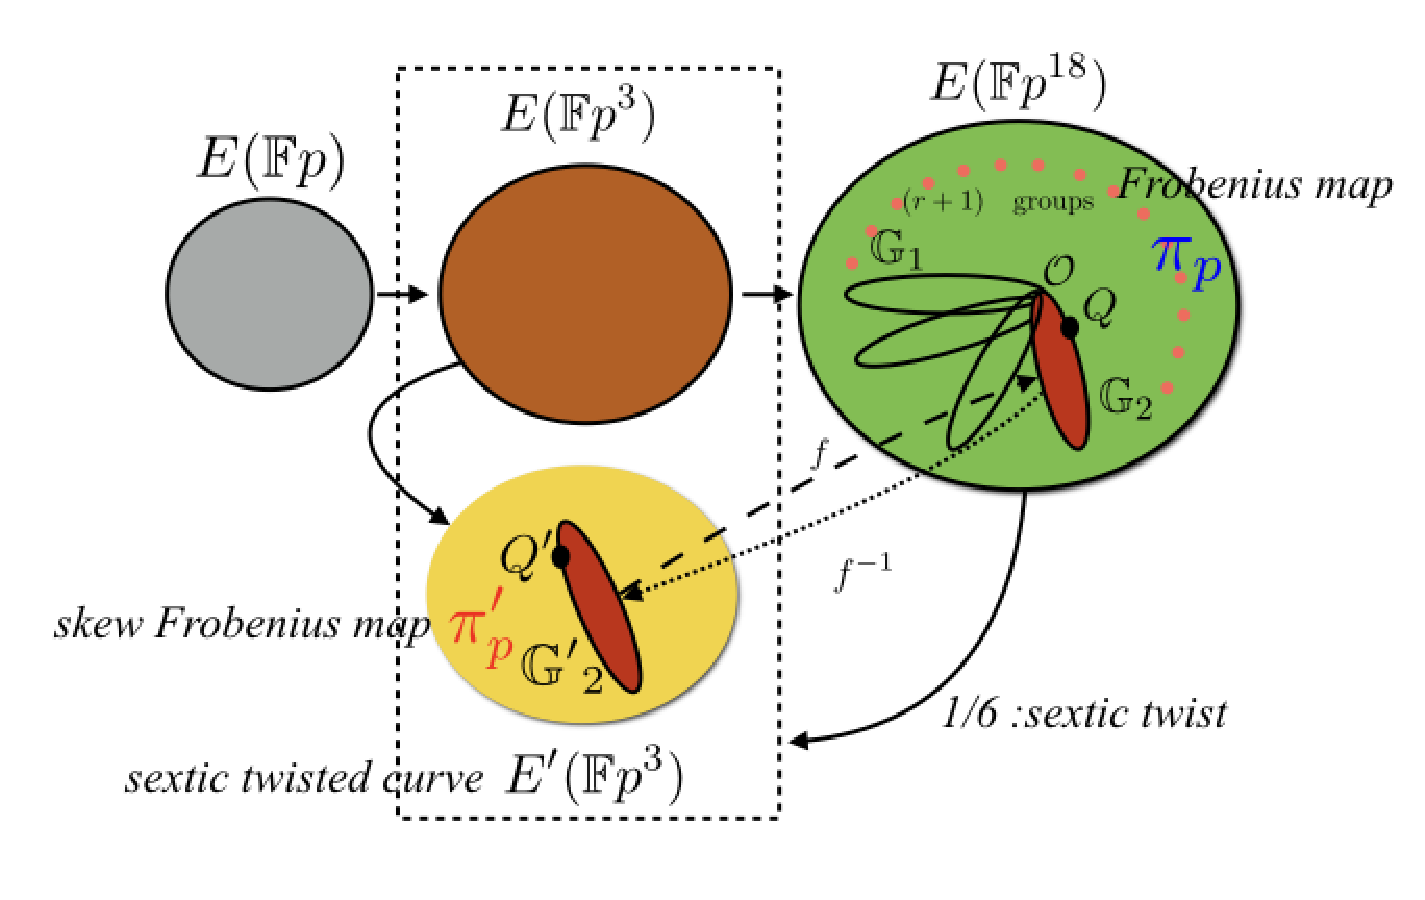
\includegraphics[width=3.5in]{sfm.eps}
\caption{\textit{sextic twist} in KSS-18 curve.}
\label{fig:sextickss18_chap_ijnc2017}
\end{figure*}

Let us consider $E$ be the KSS-18 curve in base field $\FPTH$  and $E'$ is sextic twist of $E'$ given as follows: 
\begin{eqnarray}
E:y^2 & = &x^3+b,\\
E':y^2 & = & x^3+bi, \label{eq:KSS18_Twist_chap_ijnc2017}
\end{eqnarray}
where $b \in \Fp$; $x, y, i \in \FPTH$ and basis element $i$ is the quadratic and cubic non residue in $\FPTH$.

In the context of KSS-18 curve, let us consider a rational point $Q\in \g2 \subset E(\F{p}{18})$.
$Q$ has a  special vector representation with 18 $\Fp$ elements for each $x_Q$ and $y_Q$ coordinate.
Figure \ref{fig:Q_structureKSS18_chap_ijnc2017} shows the structure of the coefficients of $Q \in \FPEN$ and its sextic twisted isomorphic rational point $Q' \in \FPTH$ in KSS-18 curve.
\begin{figure*}
\centering
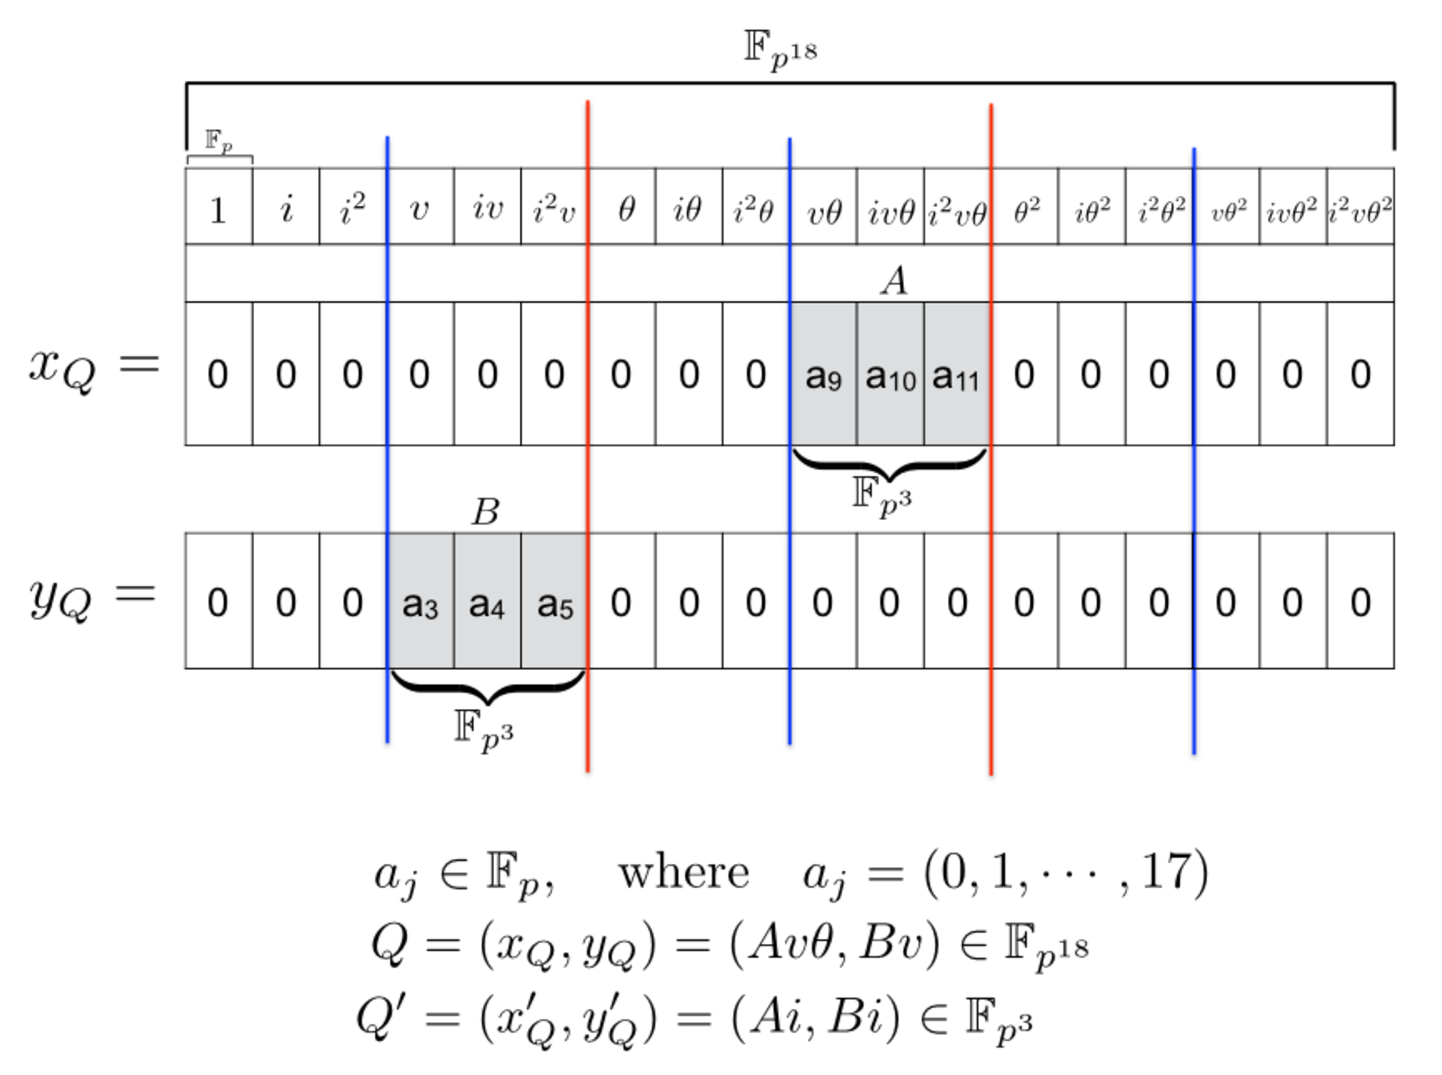
\includegraphics[width=4.5in]{structure.eps}
\caption{ $Q \in \FPEN$ and its sextic twisted isomorphic rational point $Q' \in \FPTH$ structure in KSS-18 curve.}
\label{fig:Q_structureKSS18_chap_ijnc2017}
\end{figure*}
Among 18 elements, there are 3 continuous nonzero $\Fp$ elements. The others are zero.
However, the set of these nonzero elements belongs to a $\FPTH$ field. 

This chapter considers parameter given in \tbref{table_KSS18_param_chap_ijnc2017} for KSS-18 curve where mother parameter $u=65$-bit and characteristics $p=511$-bit. In such consideration, $Q$ is given as $Q = (Av\theta, Bv)$,  showed in Figure \ref{fig:Q_structureKSS18_chap_ijnc2017}, where $A, B \in \FPTH$ and $v$ and $\theta$ are the basis elements of $\F{p}{6}$ and $\FPEN$ respectively. 

Let us consider the sextic twisted isomorphic subfield rational point of $Q$ as $Q' \in \g2' \subset E'(\F{p}{3})$.
Considering $x'$ and $y'$ as the coordinates of $Q'$, we can map the rational point $Q = (Av\theta, Bv)$  to the rational point  $Q' = (x',y')$ as follows.

Multiplying both side of \eqref{eq:KSS18_Twist_chap_ijnc2017} with $\theta^{-6}$, where $i=\theta^6$ and $v = \theta^3$.
\begin{equation}\label{eq:sextic_div_thetaKSS18_chap_ijnc2017}
E':  \Big(\frac{y}{\theta^3}\Big)^2  = \Big(\frac{x}{\theta^2}\Big)^3+ b.
\end{equation}
 $\theta^{-2}$ of  \eqref{eq:sextic_div_thetaKSS18_chap_ijnc2017} can be represented as follows:
 \begin{subequations}
 \begin{eqnarray}
 \theta^{-2} & = & i^{-1}i \theta^{-2}, \nonumber \\
 &  = & i^{-1}\theta^{4}, \label{eq:thta2_4KSS18_chap_ijnc2017}
 \end{eqnarray}
 and multiplying $i$ with both sides.
 \begin{equation} \label{eq:tthe4_2KSS18_chap_ijnc2017}
 \theta^4 = i\theta^{-2}.
 \end{equation}
Similarly $\theta^{-3}$ can be represented as follows:
 \begin{eqnarray}
 \theta^{-3} & = & i^{-1}i \theta^{-3}, \nonumber \\
 &   = & i^{-1}\theta^{3}.\label{eq:theta_3KSS18_chap_ijnc2017} 
 \end{eqnarray}
 Multiplying $i$ with both sides of \eqref{eq:theta_3KSS18_chap_ijnc2017} we get $\theta^3$ as,
 \begin{equation}\label{eq:thta_3_3KSS18_chap_ijnc2017}
 \theta^3 = i\theta^{-3},
 \end{equation}
 \end{subequations}

\subsubsection{\texorpdfstring{$Q$}{} to \texorpdfstring{$Q'$}{} Mapping in KSS-18}
Let us represent $Q = (Av\theta, Bv)$  as follows:
\begin{equation}\label{eq:map18_to3KSS18_chap_ijnc2017}
Q  =  (A\theta^4, B\theta^3), \quad \text{where $v=\theta^3$}.
\end{equation}
From \eqref{eq:tthe4_2KSS18_chap_ijnc2017} and \eqref{eq:thta_3_3KSS18_chap_ijnc2017}, we substitute $ \theta^4 = i\theta^{-2}$ and $\theta^3 = i\theta^{-3}$  in \eqref{eq:map18_to3KSS18_chap_ijnc2017}  as 
follows:
\begin{equation}\label{eq:map18_to3KSS18_chap_ijnc2017.1}
Q  =  (Ai\theta^{-2}, Bi\theta^{-3}),
\end{equation}
where $Ai = x'$ and $Bi = y'$ are the coordinates of $Q' =(x',y') \in \FPTH$. Which implies that we can map $Q \in \FPEN$ to $Q' \in \FPTH$ by first selecting the $3$ nonzero $\Fp$ coefficients of each coordinate of $Q$. Then these nonzero $\Fp$ elements form a $\FPTH$ element. After that multiplying the basis element $i$ with that $\FPTH$ element, we get the final $Q' \in \FPTH$. From the structure of $\FPEN$, given in \eqref{eq:KSS-18_towering_chap_ijnc2017}, this mapping has required no expensive arithmetic operation.  Multiplication by the basis element $i$ in $\FPTH$ can be done by 1 bitwise left shifting since $c=2$ is considered for towering in \eqref{eq:KSS-18_towering_chap_ijnc2017}.

\subsubsection{\texorpdfstring{$Q'$}{} to \texorpdfstring{$Q$}{} Mapping in KSS-18}
 The reverse mapping $Q' =(x',y') \in \FPTH$ to $Q =(Av\theta,Bv) \in \FPEN$ can be obtained as from \eqref{eq:thta2_4KSS18_chap_ijnc2017}, \eqref{eq:theta_3KSS18_chap_ijnc2017} and \eqref{eq:sextic_div_thetaKSS18_chap_ijnc2017} as follows:
 \begin{subequations}
 \begin{eqnarray}
 x i^{-1}\theta^{4} & = & Av\theta, \nonumber \\
 y i^{-1}\theta^{3} & = & Bv, \nonumber
 \end{eqnarray}
 \end{subequations}
  which resembles that $Q= (Av\theta, Bv)$. Therefore it means that multiplying $i^{-1}$ with the $Q'$ coordinates and placing the resulted coefficients in the corresponding position of the coefficients in $Q$, will map $Q'$ to $Q$.
This mapping costs one $\FPTH$ inversion of $i$ which can be pre-computed and one $\Fp$ multiplication.

\subsection{Quartic Twisted Isomorphic Mapping}
\label{sec:ch:ijnc:kss16twist_isomorphicmap}

For quartic twisted mapping first we need to obtain certain ration point  $Q \in \g2 \subset E(\FPSN)$ of subgroup order $r$. 
One necessary condition for obtaining such $Q$ is $r^2 \mid \#E(\FPSN)$, where $\#E(\FPSN)$ is the number of rational points in $E(\FPSN)$.  But it is carefully observed that $\#E(\FPSN)$ is not divisible by $r^2$ when $r$ is given by \eqref{eq:kss_16_degree_chap_ijnc2017}.
 Therefore polynomial of $r$, given in \cite{EPRINT:KacSchSco07} is divided as follows:
\begin{equation}
r(u) =  (u^8 +48u^4 +625)/61250,
\end{equation}
to make it dive  $\#E(\FPSN)$ completely.

Let us consider the rational point $Q \in \g2 \subset E(\FPSN)$ and its quartic twisted rational point $Q' \in \g2 \subset E'(\FPFR)$. Rational point $Q$ has a special vector representation given in  \tbref{table:QKSS-16_chap_ijnc2017}.

\renewcommand{\baselinestretch}{1.5}
\begin{table}[ht] 
	\begin{center}
		\caption{Vector representation of $Q = (x_Q,y_Q) \in \FPSN$}
		\resizebox{\columnwidth}{!}{
		\begin{tabular}{|c|c|c|c|c|c|c|c|c|c|c|c|c|c|c|c|c|c|}
			\hline 
			   & 1 & $\alpha$ & $\beta$ & $\alpha \beta$ & $\gamma$ & $\alpha \gamma$ & $\beta \gamma$ & $\alpha \beta \gamma$ & $\omega$ & $\alpha \omega$ & $ \beta \omega$ & $\alpha \beta \omega$ & $\gamma \omega$ & $\alpha \gamma \omega$ &$ \beta \gamma \omega$ & $\alpha \beta \gamma \omega$\\ \hline 
			$x_Q$ & 0 & 0 & 0 & 0 & $n_4$ & $n_5$ &$ n_6$ & $n_7$ & 0 & 0 & 0 & 0 & 0 & 0 & 0& 0\\ \hline 
			$y_Q$ & 0 & 0 & 0 & 0 & 0 & 0 & 0 & 0 & 0 & 0 & 0 & 0 & $n_{12}$ & $n_{13}$ & $n_{14}$ & $n_{15}$\\\hline 
		\end{tabular}\label{table:QKSS-16_chap_ijnc2017}
	}
	\end{center}
\end{table}
\renewcommand{\baselinestretch}{1.0}

From  \tbref{table:QKSS-16_chap_ijnc2017} co-ordinates of  $Q = (x_Q,y_Q) \in \FPEN$ is obtained as $Q = (x_Q,y_Q) = (\gamma x_{Q'}, \omega \gamma y_{Q'}) $ where $x_{Q'},y_{Q'}$ are the co-ordinates of the rational point $Q'$ in the twisted curve. Now let's find the twisted curve of \eqref{eq:KSS_16_trace_chap_ijnc2017} in $\FPFR$ as follows:
\begin{eqnarray}
(\omega\gamma y_{Q'} )^2 & = & (\gamma x_{Q'})^3 + a (\gamma x_{Q'}), \nonumber \\
\gamma \beta y_{Q'}^2 & = & \gamma \beta x_{Q'}^3 + a \gamma x_{Q'}, \nonumber \\
y_{Q'}^2 & = & x_{Q'}^3 + a \beta^{-1}x_{Q'}, \quad  \mbox{multiplying $(\gamma \beta)^{-1}$ both sides.}
\end{eqnarray}
 The twisted curve of $E'$ is obtained as $y^2  =  x^3 + a \beta^{-1}x$ where $\beta$ is the basis element in $\FPFR$. 
 There is a tricky part that needs attention when calculating the ECD in $E'(\FPFR)$ presented in the following equation.
 \begin{equation}
 \lambda =   (3x_{Q'}^2+\textbf{a})(2y_{Q'})^{-1},
 \end{equation}
 where $\textbf{a} \in \FPFR$, since $\textbf{a} = a \beta^{-1}$ and $\beta \in \FPFR$. The calculation of $\textbf{a} = a \beta^{-1}$
 is given as follows:
 \begin{eqnarray}
  a \beta^{-1} & = & (a + 0\alpha + 0 \beta + 0 \alpha \beta) \beta ^{-1}, \nonumber \\
  & & = z^{-1} a \alpha \beta \quad \mbox{where $\alpha^2 = z$}
 \end{eqnarray}
 
 Now let us denote the quartic mapping as follows:
 \begin{equation}
Q = (x_Q,y_Q) = (\gamma x_{Q'}, \omega \gamma y_{Q'}) \in \g2 \subset E(\FPSN)   \longmapsto  Q' = (x_{Q'},y_{Q'}) \in \g2'  \subset E'(\FPFR).  \nonumber
 \end{equation}
 
 For mapping from $Q$ to $Q'$ no extra calculation is required. By picking the non-zero coefficients  of $Q$ and placing it to the corresponding basis position is enough to get $Q'$. Similarly, re-mapping from $Q'$ to $Q$  can also be done without any calculation rather multiplying with basis elements.  

\section{Result Analysis}
The main focus of this proposed mapping is to find out the isomorphic mapping of two well-known pairing-friendly curves, KSS-16 and KSS-18. In order to determine the advantage of the proposal, this chapter has implemented 3 well-known elliptic curve scalar multiplication method named as the binary method, Montgomery ladder method, and sliding-window method.

For the experiment first we have applied the proposed mapping technique to map rational point $Q \in \g2 \subset E(\F{p}{k})$ to its isomorphic point $Q' \in \g2' \subset E'(\FPKD)$ in both KSS curves. After that we performed the scalar multiplication of $Q'$. Then the resulted points are re-mapped to $\g2$ in $\FPK$. Lets define this strategy as \textit{\textbf{with mapping}}.
On the other hand, we have performed scalar multiplication of $Q$ without mapping which is denoted as \textit{\textbf{w/o mapping}}.

In the experiment, after many careful searches, the mother parameter $u$ is selected to find out $\g2$ rational point $Q$ for KSS-18 curve. On the other hand, for KSS-16 curve, parameters are given by Loubna et al. \cite{EPRINT:GhaFou16b}.
In pairing-based cryptosystems, both KSS-16 and KSS-18 are regarded as good candidates for implementing 192-bit security.
Therefore, while choosing parameters for the experiment, this chapter has adapted 192-bit security level. 
But the main focus of this chapter is not to find out efficient parameters for certain security levels. 
The main purpose of the selected the parameters is to compare the twisted isomorphic mappings on the nominated curves at standard security levels. 

 \tbref{table_KSS18_param_chap_ijnc2017} and  \tbref{table_KSS16_param_chap_ijnc2017} show the parameters used in the experiment.
  \tbref{table_comenv_twist_chap_ijnc2017} shows the experiment environment, used to evaluate the usefulness of the proposed mapping.  
In the experiment, 100 scalar numbers of size less than order $r$ is generated randomly and then scalar multiplication is calculated for both cases. Average value of execution time in [ms] is considered for comparison. 
 \tbref{table_additional_twist_chap_ijnc2017} shows the  settings considered during the experiment.
 The comparative result is shown in  \tbref{table_opeationcomp_chap_ijnc2017}.

Parameter of KSS curves are given in decimal value used for evaluating the mapping efficiency in the experiment.

	\renewcommand{\arraystretch}{1.2}{
\begin{table}[ht]
	\centering
	\caption{KSS-18 Parameters}
	\label{table_KSS18_param_chap_ijnc2017}
	\resizebox{\columnwidth}{!}{
	\begin{tabular}{|l|l|l|}
		\hline
		$y^2 =$ & $x^3 + 11$                                                                                                                                                                                                 & bit size \\ \hline
		$u =$   & $23058430092138432950$                                                                                                                                                                                     & 65       \\ \hline
		$p=$    & \begin{tabular}[c]{@{}l@{}}$380556013753003852484338059727997572538865139076812$\\ $970560732143111526346817611942575176069026109216559$\\ $8021019048849831001675531254097766654664544068613131$\end{tabular} & 511      \\ \hline
		$r=$    & \begin{tabular}[c]{@{}l@{}}$4382120271066581232104344084955320374849908135951851$\\ $5268755202336574860904936668100704293777799119708528$\\ $7495125001$\end{tabular}                                         & 378      \\ \hline
		$t=$    & \begin{tabular}[c]{@{}l@{}}$4038507576637353290391809403638366577735736214369368$\\ $5385569578231170388739601$\end{tabular}                                                                                 & 255      \\ \hline
	\end{tabular}
}
\end{table}
}

\begin{table}[ht]
	\caption{KSS-16 Parameters}
	\label{table_KSS16_param_chap_ijnc2017}
	\resizebox{\columnwidth}{!}{
	\begin{tabular}{|l|l|l|}
		\hline
		$y^2 =$ & $x^3 + 17x$                                                                                                                                                                                               & bit size \\ \hline
		$u =$   & $1266366845779935$                                                                                                                                                                                        & 51       \\ \hline
		$p=$    & \begin{tabular}[c]{@{}l@{}}$108235379323342249430403752839634417782861787922010$\\ $5831937449880701267192580688017668298801139820714475$\\ $1031509661694254867934067997516170939905853281$\end{tabular} & 492      \\ \hline
		$r=$    & \begin{tabular}[c]{@{}l@{}}$10798667332013548302444682759479306650777434983428752$\\ $081956116352950853566245965258810783523700606376869560$\\ $4209229873$\end{tabular}                                 & 386      \\ \hline
		$t=$    & \begin{tabular}[c]{@{}l@{}}$186105672625714085505985902011330755941369113096635058$\\ $9745550013872708970$\end{tabular}                                                                                  & 247      \\ \hline
	\end{tabular}
}
\end{table}

\renewcommand{\arraystretch}{1.5}{
\begin{table}[ht]
\centering
\caption{ Computational Environment}
\label{table_comenv_twist_chap_ijnc2017}
\resizebox{\columnwidth}{!}{
\begin{tabular}{l|l|l}
\hline 
 & PC & iPhone6s \\ 
\hline \hline 
CPU {\textsuperscript{*}} & \quad 2.7 GHz Intel Core i5 \quad & \quad Apple A9 Dual-core 1.84 GHz \quad \\ 
\hline 
Memory & 16 GB & 2 GB \\ 
\hline 
OS & Mac OS X 10.12.3 &  iOS 10.2.1 \\ 
\hline 
Compiler & gcc 4.2.1 & gcc 4.2.1 \\ 
\hline 
\quad Programming Language \quad  & C & Objective-C, C \\ 
\hline 
Library & GNU MP 6.1.1\cite{gmp} & GNU MP 6.1.1 \\ 
\hline 
\multicolumn{3}{l}{\textsuperscript{*}\footnotesize{Only single core is used from two cores.}}\\
\end{tabular}
}
\end{table}
}

\renewcommand{\arraystretch}{1.3}{
\begin{table}[ht]
	\begin{center}
		\caption{Additional settings used in the experiment}
		\label{table_additional_twist_chap_ijnc2017}
		%\resizebox{\columnwidth}{!}{
		\begin{tabular}{l|l|l}
			\hline 
			 & KSS-18 & KSS-16 \\ \hline
			 Number of sample $s$& 100 & 100\\ \hline
			 Average bit size  of $s$ & 377-bit & 385-bit\\ \hline
			 Average hamming weight of s & 187 & 193\\ \hline
			 Window size for sliding window method & 4 & 4\\ \hline 
			  No. of Pre-computed ECA in sliding window  & 14 & 14\\ \hline 
			  Perceived level of security & 192-bit & 192-bit\\ \hline
		\end{tabular}
		%}
	\end{center}
\end{table}
}
 
\renewcommand{\arraystretch}{1.5}{
\begin{table}[ht]
%\renewcommand{\arraystretch}{1.3}
\centering
\caption{ Comparative result of average execution time in [ms] for scalar multiplication}
\label{table_opeationcomp_chap_ijnc2017}
\resizebox{\columnwidth}{!}{
\begin{tabular}{|l|c|c|c|c|c|c|}
\hline
& \multicolumn{6}{|c|}{\quad Average execution time [ms] comparison \quad} \\ \hline
 & \multicolumn{3}{|c|}{\quad KSS-18 \quad} & \multicolumn{3}{|c|}{\quad  KSS-16 \quad}\\ \hline
&  PC & \multicolumn{2}{|c|}{iPhone 6s}  &  PC & \multicolumn{2}{|c|}{iPhone 6s}\\ 
 \hline \hline
Binary  with mapping &  $5.7 \times 10^1 $  &  \multicolumn{2}{|c|} { $8.2 \times 10^1$} &  $1.3 \times 10^2 $  &  \multicolumn{2}{|c|} { $1.4 \times 10^2$}\\ \hline
Binary   w/o mapping  &  $1.2 \times 10^3$  &  \multicolumn{2}{|c|} { $1.8 \times 10^3$}  &  $1.2 \times 10^3 $  &  \multicolumn{2}{|c|} { $1.3 \times 10^3$}\\ \hline
Montgomery ladder  with mapping &  $7.1 \times 10^1 $  &  \multicolumn{2}{|c|} { $1.1 \times 10^2$} &  $1.7 \times 10^2$  &  \multicolumn{2}{|c|} { $1.8 \times 10^2$}\\ \hline
Montgomery ladder  w/o mapping  &  $1.5 \times 10^3$  &  \multicolumn{2}{|c|} { $ 2.4 \times 10^3$}&  $1.6 \times 10^3 $  &  \multicolumn{2}{|c|} { $1.8 \times 10^3$} \\ \hline
Sliding-window  with mapping &  $4.9 \times 10^1 $  &  \multicolumn{2}{|c|} { $7.5 \times 10^1$} &  $1.0 \times 10^2 $  &  \multicolumn{2}{|c|} { $1.3 \times 10^2$}\\ \hline
Sliding-window  w/o mapping  &  $1.0 \times 10^3$  &  \multicolumn{2}{|c|} { $1.6 \times 10^3$} &  $1.0 \times 10^3 $  &  \multicolumn{2}{|c|} { $1.2 \times 10^3$}\\ \hline
\end{tabular} 
}
\end{table}
}

Analyzing   \tbref{table_opeationcomp_chap_ijnc2017}, we can find that scalar multiplication on the sextic twisted KSS-18 curve using the proposed  mapping technique is more than 20 times faster than scalar multiplication without the proposed mapping. 
On the other hand, in the quartic twisted KSS-16 curve, scalar multiplication becomes at most 10 times faster after applying proposed mapping techniques than no mapping. 
Another important difference is sextic twisted mapped points take less  time for scalar multiplication in both experiment environments. Therefore we can certainly say sextic twist over KSS-18 is more efficient than the quartic twisted KSS-16 curve for implementing  pairing operations.

In the experiment we have used two execution environments; such as PC and iPhone with different CPU frequencies. 
In both environments only one processor core is utilized.
 The ratio of CPU frequencies of  iPhone and PC is about $1.84 / 2.7 \approx 0.68$. 
The result  shows that the ratio of execution time of PC and iPhone without mapping  for KSS-18 curve is around $0.62$ to $0.66$.
Which is close to CPU frequency ratio.
On the other hand, the ratio of execution time with mapping  of KSS-18 curve is also around $0.6$. 
For KSS-16 curve, the ratio with no mapping case is more than $0.8$ and for mapping case it is around $0.7$ to $0.9$.   
Since PC and iPhone has different processor architectures therefore it's frequency ratio has modest relation with the execution time ratio. 
The ratio may also be effected by the other processes, running in certain environment during the experiment time.

The main focus of this experiment is to evaluate the  acceleration ratio of scalar multiplication by applying the proposed mapping on $\g2$ rational point group of the nominated KSS curves. The experiment does not focus on efficiently implementing scalar multiplication for certain environment. There are other pairing-friendly curves such as BLS-12, BLS-24 \cite{JC:FreScoTes10} where sextic twist is available. As our future work, we will try to apply the proposed mapping on those curves.

\section{Conclusion}
In this chapter, we have demonstrated isomorphic mapping procedure of $\g2$ rational point group to its sextic and quartic twisted subfield isomorphic rational point group $\g2'$  and its reverse mapping for KSS-18 and KSS-16 curves in the context of Ate-based pairing. 

We have also evaluated the advantage of such mapping by applying binary scalar multiplication, Montgomery ladder, and sliding- window method on twisted isomorphic rational points in $\g2'$. 
Then result of  scalar multiplication in $\g2'$ can accelerate the scalar multiplication in $\g2 \subset E(\FPEN)$ by   20 to 10 times than scalar multiplication of $\g2$ rational point directly in $\FPEN$ and $\FPSN$. 
